%%%%%%%%%%%%%%%%%%%%%%%%%%%%%%%%%%%%%%%%%%%%%%%%%%%%%%%%%%%%%%%%%%%%%%%%%%
%
% 	Template for seminar reports
%
%%%%%%%%%%%%%%%%%%%%%%%%%%%%%%%%%%%%%%%%%%%%%%%%%%%%%%%%%%%%%%%%%%%%%%%%%%

%%%%%%%%%%%%%%%%%%%%%%%%%%%%%%%%%%%%%%%%%%%%%%%%%%%%%%%%%%%%%%%%%%%%%%%%%%
% 	Include layout and macros
%%%%%%%%%%%%%%%%%%%%%%%%%%%%%%%%%%%%%%%%%%%%%%%%%%%%%%%%%%%%%%%%%%%%%%%%%%


%% This LaTeX template is based on the following example file included in the ieeetran
%% package:
%% bare_conf.tex 
%% V1.2
%% 2002/11/18
%% by Michael Shell
%% mshell@ece.gatech.edu
%% (requires IEEEtran.cls version 1.6b or later) with an IEEE conference paper.


% Note that the a4paper option is mainly intended so that authors in
% countries using A4 can easily print to A4 and see how their papers will
% look in print. Authors are encouraged to use U.S. letter paper when 
% submitting to IEEE. Use the testflow package mentioned above to verify
% correct handling of both paper sizes by the author's LaTeX system.
%
% Also note that the "draftcls" or "draftclsnofoot", not "draft", option
% should be used if it is desired that the figures are to be displayed in
% draft mode.
%
% This paper can be formatted using the peerreviewca
% (instead of conference) mode.
\documentclass[conference, a4paper]{Style/IEEEtran-modified}
% If the IEEEtran.cls has not been installed into the LaTeX system files, 
% manually specify the path to it:
% \documentclass[conference]{../sty/IEEEtran} 

\IEEEoverridecommandlockouts

% some very useful LaTeX packages include:

\usepackage{cite}       % Written by Donald Arseneau
                        % V1.6 and later of IEEEtran pre-defines the format
                        % of the cite.sty package \cite{} output to follow
                        % that of IEEE. Loading the cite package will
                        % result in citation numbers being automatically
                        % sorted and properly "ranged". i.e.,
                        % [1], [9], [2], [7], [5], [6]
                        % (without using cite.sty)
                        % will become:
                        % [1], [2], [5]--[7], [9] (using cite.sty)
                        % cite.sty's \cite will automatically add leading
                        % space, if needed. Use cite.sty's noadjust option
                        % (cite.sty V3.8 and later) if you want to turn this
                        % off. cite.sty is already installed on most LaTeX
                        % systems. The latest version can be obtained at:
                        % http://www.ctan.org/tex-archive/macros/latex/contrib/supported/cite/

%\usepackage{graphicx}  % Written by David Carlisle and Sebastian Rahtz
                        % Required if you want graphics, photos, etc.
                        % graphicx.sty is already installed on most LaTeX
                        % systems. The latest version and documentation can
                        % be obtained at:
                        % http://www.ctan.org/tex-archive/macros/latex/required/graphics/
                        % Another good source of documentation is "Using
                        % Imported Graphics in LaTeX2e" by Keith Reckdahl
                        % which can be found as esplatex.ps and epslatex.pdf
                        % at: http://www.ctan.org/tex-archive/info/
% NOTE: for dual use with latex and pdflatex, instead load graphicx like:
\ifx\pdfoutput\undefined
	\usepackage{graphicx}
\else
	\usepackage[pdftex]{graphicx}
\fi

% However, be warned that pdflatex will require graphics to be in PDF
% (not EPS) format and will preclude the use of PostScript based LaTeX
% packages such as psfrag.sty and pstricks.sty. IEEE conferences typically
% allow PDF graphics (and hence pdfLaTeX). However, IEEE journals do not
% (yet) allow image formats other than EPS or TIFF. Therefore, authors of
% journal papers should use traditional LaTeX with EPS graphics.
%
% The path(s) to the graphics files can also be declared: e.g.,
% \graphicspath{{../eps/}{../ps/}}
% if the graphics files are not located in the same directory as the
% .tex file. This can be done in each branch of the conditional above
% (after graphicx is loaded) to handle the EPS and PDF cases separately.
% In this way, full path information will not have to be specified in
% each \includegraphics command.
%
% Note that, when switching from latex to pdflatex and vice-versa, the new
% compiler will have to be run twice to clear some warnings.
\graphicspath{{figures/}}


%\usepackage{psfrag}    % Written by Craig Barratt, Michael C. Grant,
                        % and David Carlisle
                        % This package allows you to substitute LaTeX
                        % commands for text in imported EPS graphic files.
                        % In this way, LaTeX symbols can be placed into
                        % graphics that have been generated by other
                        % applications. You must use latex->dvips->ps2pdf
                        % workflow (not direct pdf output from pdflatex) if
                        % you wish to use this capability because it works
                        % via some PostScript tricks. Alternatively, the
                        % graphics could be processed as separate files via
                        % psfrag and dvips, then converted to PDF for
                        % inclusion in the main file which uses pdflatex.
                        % Docs are in "The PSfrag System" by Michael C. Grant
                        % and David Carlisle. There is also some information 
                        % about using psfrag in "Using Imported Graphics in
                        % LaTeX2e" by Keith Reckdahl which documents the
                        % graphicx package (see above). The psfrag package
                        % and documentation can be obtained at:
                        % http://www.ctan.org/tex-archive/macros/latex/contrib/supported/psfrag/

%\usepackage{subfigure} % Written by Steven Douglas Cochran
                        % This package makes it easy to put subfigures
                        % in your figures. i.e., "figure 1a and 1b"
                        % Docs are in "Using Imported Graphics in LaTeX2e"
                        % by Keith Reckdahl which also documents the graphicx
                        % package (see above). subfigure.sty is already
                        % installed on most LaTeX systems. The latest version
                        % and documentation can be obtained at:
                        % http://www.ctan.org/tex-archive/macros/latex/contrib/supported/subfigure/

%\usepackage{url}       % Written by Donald Arseneau
                        % Provides better support for handling and breaking
                        % URLs. url.sty is already installed on most LaTeX
                        % systems. The latest version can be obtained at:
                        % http://www.ctan.org/tex-archive/macros/latex/contrib/other/misc/
                        % Read the url.sty source comments for usage information.

%\usepackage{stfloats}  % Written by Sigitas Tolusis
                        % Gives LaTeX2e the ability to do double column
                        % floats at the bottom of the page as well as the top.
                        % (e.g., "\begin{figure*}[!b]" is not normally
                        % possible in LaTeX2e). This is an invasive package
                        % which rewrites many portions of the LaTeX2e output
                        % routines. It may not work with other packages that
                        % modify the LaTeX2e output routine and/or with other
                        % versions of LaTeX. The latest version and
                        % documentation can be obtained at:
                        % http://www.ctan.org/tex-archive/macros/latex/contrib/supported/sttools/
                        % Documentation is contained in the stfloats.sty
                        % comments as well as in the presfull.pdf file.
                        % Do not use the stfloats baselinefloat ability as
                        % IEEE does not allow \baselineskip to stretch.
                        % Authors submitting work to the IEEE should note
                        % that IEEE rarely uses double column equations and
                        % that authors should try to avoid such use.
                        % Do not be tempted to use the cuted.sty or
                        % midfloat.sty package (by the same author) as IEEE
                        % does not format its papers in such ways.

\usepackage{amsmath}    % From the American Mathematical Society
                        % A popular package that provides many helpful commands
                        % for dealing with mathematics. Note that the AMSmath
                        % package sets \interdisplaylinepenalty to 10000 thus
                        % preventing page breaks from occurring within multiline
                        % equations. Use:
\interdisplaylinepenalty=2500
                        % after loading amsmath to restore such page breaks
                        % as IEEEtran.cls normally does. amsmath.sty is already
                        % installed on most LaTeX systems. The latest version
                        % and documentation can be obtained at:
                        % http://www.ctan.org/tex-archive/macros/latex/required/amslatex/math/



% Other popular packages for formatting tables and equations include:

%\usepackage{array}
% Frank Mittelbach's and David Carlisle's array.sty which improves the
% LaTeX2e array and tabular environments to provide better appearances and
% additional user controls. array.sty is already installed on most systems.
% The latest version and documentation can be obtained at:
% http://www.ctan.org/tex-archive/macros/latex/required/tools/

% Mark Wooding's extremely powerful MDW tools, especially mdwmath.sty and
% mdwtab.sty which are used to format equations and tables, respectively.
% The MDWtools set is already installed on most LaTeX systems. The lastest
% version and documentation is available at:
% http://www.ctan.org/tex-archive/macros/latex/contrib/supported/mdwtools/


% V1.6 of IEEEtran contains the IEEEeqnarray family of commands that can
% be used to generate multiline equations as well as matrices, tables, etc.


% Also of notable interest:

% Scott Pakin's eqparbox package for creating (automatically sized) equal
% width boxes. Available:
% http://www.ctan.org/tex-archive/macros/latex/contrib/supported/eqparbox/



% Notes on hyperref:
% IEEEtran.cls attempts to be compliant with the hyperref package, written
% by Heiko Oberdiek and Sebastian Rahtz, which provides hyperlinks within
% a document as well as an index for PDF files (produced via pdflatex).
% However, it is a tad difficult to properly interface LaTeX classes and
% packages with this (necessarily) complex and invasive package. It is
% recommended that hyperref not be used for work that is to be submitted
% to the IEEE. Users who wish to use hyperref *must* ensure that their
% hyperref version is 6.72u or later *and* IEEEtran.cls is version 1.6b 
% or later. The latest version of hyperref can be obtained at:
%
% http://www.ctan.org/tex-archive/macros/latex/contrib/supported/hyperref/
%
% Also, be aware that cite.sty (as of version 3.9, 11/2001) and hyperref.sty
% (as of version 6.72t, 2002/07/25) do not work optimally together.
% To mediate the differences between these two packages, IEEEtran.cls, as
% of v1.6b, predefines a command that fools hyperref into thinking that
% the natbib package is being used - causing it not to modify the existing
% citation commands, and allowing cite.sty to operate as normal. However,
% as a result, citation numbers will not be hyperlinked. Another side effect
% of this approach is that the natbib.sty package will not properly load
% under IEEEtran.cls. However, current versions of natbib are not capable
% of compressing and sorting citation numbers in IEEE's style - so this
% should not be an issue. If, for some strange reason, the user wants to
% load natbib.sty under IEEEtran.cls, the following code must be placed
% before natbib.sty can be loaded:
%
% \makeatletter
% \let\NAT@parse\undefined
% \makeatother
%
% Hyperref should be loaded differently depending on whether pdflatex
% or traditional latex is being used:
%
%\ifx\pdfoutput\undefined
%\usepackage[hypertex]{hyperref}
%\else
%\usepackage[pdftex,hypertexnames=false]{hyperref}
%\fi
%
% Pdflatex produces superior hyperref results and is the recommended
% compiler for such use.



% *** Do not adjust lengths that control margins, column widths, etc. ***
% *** Do not use packages that alter fonts (such as pslatex).         ***
% There should be no need to do such things with IEEEtran.cls V1.6 and later.

% Packages to load
\usepackage[english]{babel}
%%% Support some german text
\usepackage{ngerman}
\usepackage[latin1]{inputenc}   % für Umlaute
%%%
% \usepackage[utf8]{inputenc}
\usepackage[T1]{fontenc}
\usepackage{microtype}
%%% Todo margin notes
\usepackage{todonotes}
% \usepackage[disable]{todonotes}
%%%


% Simple helpful macro to deal with TODO parts in text
\newcommand{\TODO}{TODO\todo{\#}: }

%%%%%%%%%%%%%%%%%%%%%%%%%%%%%%%%%%%%%%%%%%%%%%%%%%%%%%%%%%%%%%%%%%%%%%%%%%
% 	Page numbering (not on first page)
%%%%%%%%%%%%%%%%%%%%%%%%%%%%%%%%%%%%%%%%%%%%%%%%%%%%%%%%%%%%%%%%%%%%%%%%%%
\pagestyle{empty}

%%%%%%%%%%%%%%%%%%%%%%%%%%%%%%%%%%%%%%%%%%%%%%%%%%%%%%%%%%%%%%%%%%%%%%%%%%
% 	Correct bad hyphenation here
%%%%%%%%%%%%%%%%%%%%%%%%%%%%%%%%%%%%%%%%%%%%%%%%%%%%%%%%%%%%%%%%%%%%%%%%%%

\hyphenation{}

%%%%%%%%%%%%%%%%%%%%%%%%%%%%%%%%%%%%%%%%%%%%%%%%%%%%%%%%%%%%%%%%%%%%%%%%%%
% 	Begin of the document
%%%%%%%%%%%%%%%%%%%%%%%%%%%%%%%%%%%%%%%%%%%%%%%%%%%%%%%%%%%%%%%%%%%%%%%%%%

\begin{document}

%%%%%%%%%%%%%%%%%%%%%%%%%%%%%%%%%%%%%%%%%%%%%%%%%%%%%%%%%%%%%%%%%%%%%%%%%%
% 	Paper title
%%%%%%%%%%%%%%%%%%%%%%%%%%%%%%%%%%%%%%%%%%%%%%%%%%%%%%%%%%%%%%%%%%%%%%%%%%

\title{How runtime systems can support resource awareness in HPC: the HPX case}

%%%%%%%%%%%%%%%%%%%%%%%%%%%%%%%%%%%%%%%%%%%%%%%%%%%%%%%%%%%%%%%%%%%%%%%%%%
% 	Author names and affiliations 
%		-	multiple columns for up to three different affilitations are separated 
%			by \and
%		- for over three affiliations, refer to ieeetran howto
%%%%%%%%%%%%%%%%%%%%%%%%%%%%%%%%%%%%%%%%%%%%%%%%%%%%%%%%%%%%%%%%%%%%%%%%%%

\author{
\authorblockN{Tommaso Bianucci}
\authorblockA{Fakult�t f�r Informatik\\Technische Universit�t M�nchen\\
Email: bianucci@in.tum.de} 
%\and
%\authorblockN{}
%\authorblockA{}
}

%%%%%%%%%%%%%%%%%%%%%%%%%%%%%%%%%%%%%%%%%%%%%%%%%%%%%%%%%%%%%%%%%%%%%%%%%%
% 	Special paper note (appears between title and authors) 
%%%%%%%%%%%%%%%%%%%%%%%%%%%%%%%%%%%%%%%%%%%%%%%%%%%%%%%%%%%%%%%%%%%%%%%%%%

\specialpapernotice{Seminar Future Trends in High Performance Computing}

%%%%%%%%%%%%%%%%%%%%%%%%%%%%%%%%%%%%%%%%%%%%%%%%%%%%%%%%%%%%%%%%%%%%%%%%%%
% 	Make title area 
%%%%%%%%%%%%%%%%%%%%%%%%%%%%%%%%%%%%%%%%%%%%%%%%%%%%%%%%%%%%%%%%%%%%%%%%%%

\maketitle

%%%%%%%%%%%%%%%%%%%%%%%%%%%%%%%%%%%%%%%%%%%%%%%%%%%%%%%%%%%%%%%%%%%%%%%%%%
% 	For page number on first page
%%%%%%%%%%%%%%%%%%%%%%%%%%%%%%%%%%%%%%%%%%%%%%%%%%%%%%%%%%%%%%%%%%%%%%%%%%

%\thispagestyle{plain}

%%%%%%%%%%%%%%%%%%%%%%%%%%%%%%%%%%%%%%%%%%%%%%%%%%%%%%%%%%%%%%%%%%%%%%%%%%
% 	Abstract 
%%%%%%%%%%%%%%%%%%%%%%%%%%%%%%%%%%%%%%%%%%%%%%%%%%%%%%%%%%%%%%%%%%%%%%%%%%


\begin{abstract}
Resource awareness is the ability of a program to dinamically read the state of the resources it consumes and to adapt its execution accordingly.
This awareness can be exploited to achieve a more efficient resource usage, reduce overheads, improve performance and optimize energy consumption.
As HPC systems grow in size and complexity, resource awareness can also offer a way to reduce the effort required for tuning and portability.
As applications use runtime systems for parallelization, there is the need for runtime systems to support and expose resource awareness in an efficient and integrated way.
HPX is a modern C++ runtime system for high-performance task-based parallelization which is, to some degree, resource aware and adaptive by design.
It supports load-aware task scheduling and a powerful performance monitoring framework which can be used for runtime introspection and for building dynamic resource management heuristics.
Recent research efforts also show how HPX can support dynamic task grain size control and how HPX parallel algorithms can be dynamically tuned by using a mix of compile-time and runtime information for better performance.
\end{abstract}

~\\~
%%%%%%%%%%%%%%%%%%%%%%%%%%%%%%%%%%%%%%%%%%%%%%%%%%%%%%%%%%%%%%%%%%%%%%%%%%
% 	Keywords 
%%%%%%%%%%%%%%%%%%%%%%%%%%%%%%%%%%%%%%%%%%%%%%%%%%%%%%%%%%%%%%%%%%%%%%%%%%

\begin{keywords}
Resource awareness, HPX, task-based parallelism, HPC
\end{keywords}


%%%%%%%%%%%%%%%%%%%%%%%%%%%%%%%%%%%%%%%%%%%%%%%%%%%%%%%%%%%%%%%%%%%%%%%%%%
% 	Sections, Subsections,...
%%%%%%%%%%%%%%%%%%%%%%%%%%%%%%%%%%%%%%%%%%%%%%%%%%%%%%%%%%%%%%%%%%%%%%%%%%


~\\~
\section{Introduction}
\enlargethispage{-1\baselineskip} % Ensure no RIGHINO/VEDOVA on newpage!
% The world of scientific computing and, specifically, High Performance Computing has undergone a deep revolution in the last 20 years.
% The time when it was possible to improve software performance and time to solution just by using newer and faster hardware is long gone due to the halt in frequency increase in processors that happened around year 2000 \todo{see free lunch is over}.
% This required a paradigm shift in how software is designed and implemented, in order to make it able to leverage the increasing parallelism delivered by current processing hardware units.
% However, the time of being able to achieve good parallel performance on very high scale problems by using MPI+X, with X being any means for intra-node parallelization\footnote{as e.g. OpenMP or CUDA}, and careful programming seems to be coming to an end soon too\todo{find some cit supporting this}\cite{heller2017hpx}.

Current supercomputers are approaching the long awaited exascale and are characterized by millions of cores, distributed not only over nodes but also over several different architectures as many-core CPUs, GPUs, gpGPUs\footnote{General Purpose GPUs.} and FPGAs\footnote{Field Programmable Gate Arrays.}.
The number of processing units and their heterogeneity makes it extremely complex to program them using static and manual resource allocation paradigms.

Furthermore, many important application classes are characterized by highly unbalanced execution trees (e.g. AMR\footnote{Adaptive Mesh Refinement} strategies): in these cases the resource requirements and the load are inherently unbalanced and difficult to mitigate.
This impacts on parallel performance and causes a sub-optimal resource usage, where most of the processes sit waiting for the few more expensive ones to finish their respective computations.

Solving this problem and the ability to effectively and efficiently scale computations up to the current supercomputer capabilities requires the possibility to change resource allocation and requirements dynamically.

This is where \emph{resource aware computing} comes into play: as a general concept, we would like applications and systems to be able to react to different load distributions and resource availability directly at runtime. Resource awareness can be seen at all levels of a system: starting from hardware and operating system, through the runtime environment of choice and the application. But resource awareness can also be facilitated and supported by the choice of appropriate algorithms and programming models.

% The current predominant approach in HPC is to use the Bulk Synchronous Parallel (BSP) \todo{Maybe better to talk about CSP (communicating sequential processes)?} computing model\cite{cheatham1996bulk}. This is is based on splitting the computation in \emph{supersteps}: each superstep can be parallelized on several threads which then undergo a global synchronization (a barrier) at the end. Wiring all these supersteps together in the right order then yields the entire computation, which is essentially retaining its high-level sequentiality.
The current predominant programming model in HPC is to use a \emph{fork-join} model for shared memory parallelization together with a \emph{Communicating Sequential Processes (CSP)}\cite{hoare1978communicating} model for distributed memory parallelization. This is done in practice by leveraging respectively OpenMP and MPI.
This hybrid model involves many synchronization barriers at the boundaries of parallel regions, which are often global or involve a high number of parallel processes.

% While this model was proposed in an effort to standardize the approach to parallelization in the nineties, it is easy to see its limitations in today's HPC landscape.
Such barriers quickly become bottlenecks when the number of processes increase and in case of any load unbalance, since all threads will have to wait for the slowest one to complete its tasks (Figure \ref{fig:globalBarriers}).
As foreseen by the Exascale Study Group in 2008: ``Somewhere between Petascale and Exascale computing [...] the MPI model may find its limit''.\cite{bergman2008exascale}
% This can partly be solved by leveraging clever decompositions into processes and by performing synchronization barriers on specific subsets of them. However the complexity of these approaches quickly becomes extremely challanging to manage and, most importantly, they require specific solutions to be carefully crafted within each application, therefore requiring the developer to create ad-hoc solutions which cannot be reused.

In order to solve this problem, alternative runtime systems based on the Asynchronous Many Tasks (AMT) model are being proposed\cite{heller2017hpx}. This approach is based on splitting the computation in many fine-grained \emph{tasks} and in defining their precise dependencies on each other.
It is then the job of the runtime system to make sure each dependency is satisfied by using the appropriate synchronization.
In this way we obtain an execution graph where each task will only wait for the completion of the tasks it depends on before starting. We thus lose the concept of 
% sister threads starting in parallel after a global barrier 
a group of threads executing in parallel between global barriers
and, most importantly, we lose the global barriers themselves.

% The gain in time-to-solution obtained by using AMT might not be high or it might even be non-existent, however if we couple AMT with the ability to dynamically allocate and release resources as needed (basically according to the width of the execution graph), we can achieve a much better resource utilization and, ultimately, throughput from a computing centre perspective.

Task-based semantic has been integrated in a variety of runtimes libraries, such as Intel TBB\cite{contreras2008characterizing}, Charm++\cite{charmpp}, Qthreads\cite{qthreads} and HPX\cite{heller2017hpx}. Also OpenMP has added extensions for task-based parallelism starting from its 3.0 release\cite{omp30}.
In order to achieve true scalability, a runtime supporting task-based parallelism must be able to support it in a massive fashion. This requires the ability to schedule tasks without allocating a new OS thread for each of them, which would be infeasible, but it also requires adaptive resource management and task scheduling in order to ensure the required performance.

In this work I review the general concepts of resource awareness (\ref{sec:resourceAwareness}), then I review the \emph{High Performance paralleX (HPX)} runtime system, its design and its features (\ref{sec:hpx}). Then I discuss how HPX can support resource awareness and its limitations in this (\ref{sec:hpxRAC}).
In section \ref{sec:examples} I also present 
% how a simple CFD solver\todo{check if better a simpler example}, previously parallelized with MPI, can be ported to HPX and I will compare briefly the performance of the two approaches when run on a shared memory machine.
a basic example of HPX code and I briefly compare its performance against PThreads and OpenMP parallelizations on a shared memory machine.

\begin{figure}[t]
 	\begin{center}
 		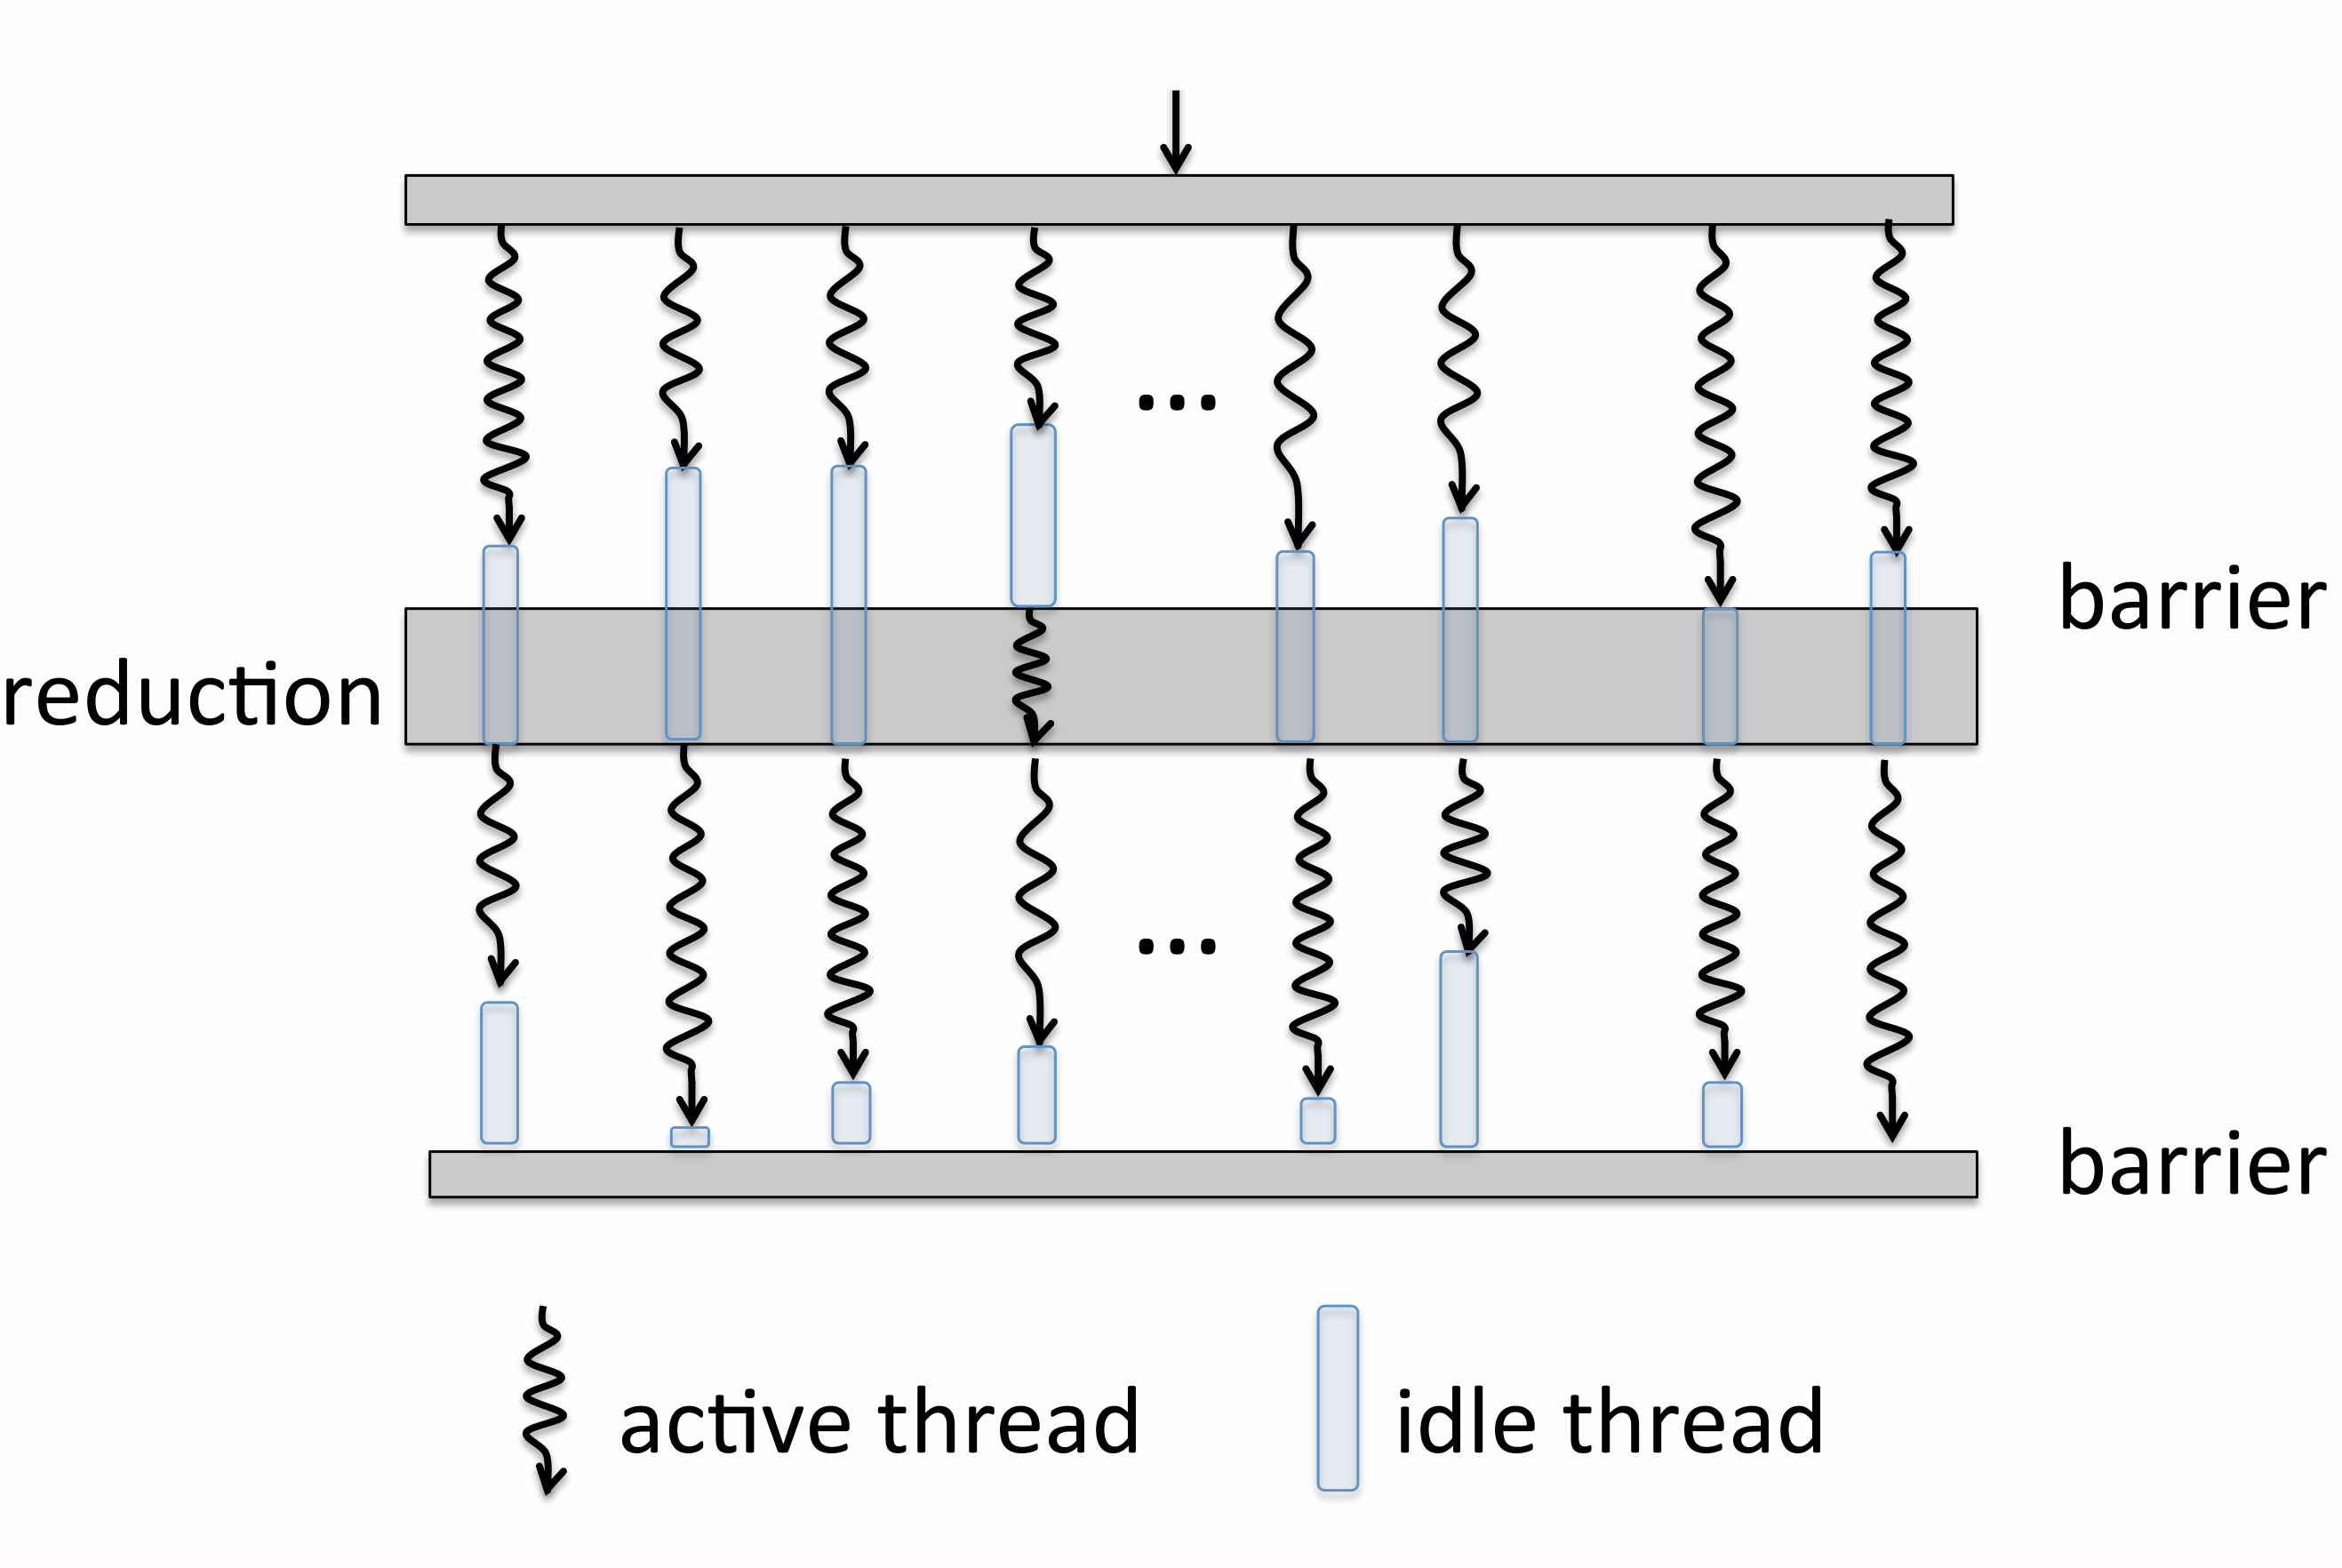
\includegraphics[scale=0.09]{Figures/globalBarriersAndThreadIdleTime.png}
 		\caption{Global barriers and thread idle time\protect\cite{grubel2016dynamic}.
 		This is a representation of how global barriers cause idling on threads with unbalanced workload.
 		We can also see how, during a reduction, just one thread actually operates it while all the others are idle.}
 		\label{fig:globalBarriers}
 	\end{center}
\end{figure}

%eof



\section{Resource Awareness} \label{sec:resourceAwareness}

\emph{Resource aware computing (RAC)}, also referred to as \emph{runtime adaptivity} or \emph{elasticity}, comprises a broad spectrum of techniques aimed at achieving runtime adaptivity in resource allocation and usage. The definition of resource is very broad and comprises computational units, memory, bus or network bandwidth, I/O.

The key point of resource awareness is to make the application and the system aware, at runtime, of what resources are available and in what amount and how much of these resources is currently in use.

This is opposed to the standard approach in which software is optimized to a certain degree for specific constraints and amount of resources before compilation occurs.
Also, in the current standard approach the program is statically assigned a certain amount of resources (e.g. processors) at the beginning of its run and this amount stays assigned to the program also in phases when it does not need them. This causes the resource to be unavailable to other processes while it is, in fact, idle.

Resource awareness can be seen at several levels and in different contexts.

In embedded computing and in the context of \emph{Multi-Processor System on Chip (MPSoC)} the aim is to ``deal with increasing imperfections such as process variation, fault rates, aging effects, and power as well as thermal problems''\cite{hannig2011resource}. Interesting research efforts are going in the direction of the \emph{Invasive Computing}\cite{teich2011invasive} paradigm: in this model a program can dynamically explore and claim resources in its neighborhood in order to increase its parallelism, in a phase called \emph{invasion}; then, when a lower degree of parallelism is needed, it can autonomously release these resources through an opposite process called \emph{retreat}, making the resources available to other applications.

In the context of a runtime system or a single parallel application we can see resource awareness in introducing the ability to steer the execution in a way to meet resource availability. Task scheduling takes a major role within runtime systems, as we will later see for HPX in section \ref{sec:hpxRAC}. The ability to query the state of the resources at runtime can also lead to resource awareness in applications: it can be used for runtime tuning of execution parameters in order to achieve, e.g. a better time to solution or a higher energy efficiency. One example for this is automatic tuning of task grain size\cite{grubel2016dynamic}.

At the computing facility level, resource awareness can instead be used for more efficient scheduling of jobs, in order to get a better utilization of resources and more predictable power requirements. One interesting example in this direction comes again from invasive computing: here an extension of MPI supporting invasive operations has been developed in order to allow varying resource utilization at runtime\cite{urena2012invasive}. The research effort is currently on developing a process manager capable of leveraging this elasticity for a better machine utilization and, ultimately, an improved throughput.

% \begin{figure}[h]%
%  	\begin{center}%
%  		\includegraphics[scale=0.1]{Figures/figure1.png}%
%  		\caption{Baum}\label{fig:baum}%
%  	\end{center}%
% \end{figure}

% \begin{table}[h]%
%  	\begin{center}%
% 		\caption{Beispieltabelle}\label{tab:example}%
% 	 	\begin{tabular}{c|c}%
%  			Spalte1 & Spalte2\\
%  			\hline
%  			0 & 1\\
%  		\end{tabular}%
%  	\end{center}%
% \end{table}


\section{HPX}
HPX is a C++ library and runtime system for task-based parallellization. It treats both intra- and inter-node parallelization within an homogeneus interface and it adheres to the C++11/14 standard, which introduced basic support for task-based parallelism.

It features a global address space, the ability to migrate work remotely in the proximity of data, and it supports task dependencies and continuations. It also delivers a powerful performance monitoring system which allows a program to query various performance metrics at runtime and to react accordingly.

\subsection{The ParalleX execution model}\label{subs:parallexModel}
HPX implements the ParalleX \cite{kaiser2009parallex} execution model, which leverages medium- and fine-grained task parallelism and aims at optimizing both parallel efficiency and programmability of parallel code.

The key highlights of this model are:
\begin{description}
	\item [Asynchronous task execution] Functions are meant to be called asynchronously and to yield a proxy for the actual return value. Such a proxy is called a \emph{future}. The program will need to synchronize only when the actual return value is needed, e.g. for a later computation. If the task was able to complete between the asynchronous call and the synchronization step, then no waiting time is needed.
	\item [Lightweight synchronization] Not only we can use futures but we can also make an asynchronous call depend on one or several futures: this enables the runtime system to keep track of the actual dependencies and removes the need for expensive synchronization mechanisms, such as global barriers.
	\item [Active Global Address Space (AGAS)] ParalleX features a global address space abstraction service. This address space spans all the available hardware entities, called \emph{localities}.
	What is special about it is that it is not a \emph{partitioned} global address space (PGAS): in PGAS the global address space is statically partitioned across the available localities and moving an object to a different locality requires a change of its address; in AGAS the address space is dynamically and adaptively mapped to the underlying localities, allowing transparent migration of objects across localities while they can still retain their \emph{global identifier (GID)}.
	\item [Message-driven queue-based scheduling] When a task execution is requested, which may be on any remote locality, an active message, called \emph{parcel}, is sent to the target locality. This triggers the creation of a \emph{PX-Thread}\footnote{From now on PX-Threads will be referred to just as \emph{threads}.}, which will be queued and then scheduled for execution on the OS thread(s) managed by the target locality. This form of message passing is therefore not limited to data and it does not require explicit receive operations to be invoked on the target side. The queuing and scheduling is designed in a way to allow for idling processors or cores to \emph{steal} work from the queues of other ones: this allows for efficient load balancing and prevents starvation\todo{maybe explain starvation}.
\end{description}

% This clearly differentiates from the usual \emph{Single Program Multiple Data (SPMD)} approach used in MPI and OpenMP, as there is no need to explicitly take care 

\subsection{HPX high-level architecture}
HPX implements the ParalleX model as a C++ library adhering to C++11/14 standard interfaces for task-based parallelism.
It aims to address the four main factors that prevent scaling in scaling-impaired applications, which are referred to as \emph{SLOW}\cite{kaiser2014hpx}:
\begin{description}
	\item [Starvation] Not all resources are fully utilized because of a lack of enough concurrent work to execute.
	\item [Latencies] Intrinsic delays in accessing remote resources.
	\item [Overheads] The overheads of parallelization, i.e. the work required for management of the parallel computation and any extra work which would not be necessary in a sequential version.
	\item [Waiting for contention resolution] Any delay caused by oversubscription of shared resources.
\end{description}

HPX tries to deal with the above problems by embracing the following design principles: focus on latency hiding instead of latency avoidance, embrace fine-grained parallelism, leverage constraint based synchronization, use adaptive locality control instead of static data distribution, move work to data instead of data to work and embrace message driven computation instead of message passing.\cite{kaiser2014hpx}

[\TODO we must add something more here...]

The high-level fundamental components of HPX are:

\paragraph{Threads \& Scheduling}
When a new thread is created, HPX queues it at an appropriate locality and it then schedules it according to configurable policies. The scheduling is cooperative, i.e. non-preemptive, since preemption and the overhead associated to content switches would not make sense in the context of a single application. Threads are scheduled onto a pool of OS threads, which are usually one per core, whitout requiring any kernel transition and thus removing all the overhead associated to the creation of OS threads.

\paragraph{Parcels}
Parcels are the HPX implementation of active messages, i.e. messages which can not only deliver data but also trigger execution of methods on remote localities.
Parcels carry the GID of the remote action, arguments for the action and, if required, a continuation.

\paragraph{Local Control Objects}
``Local Control Objects (LCOs) control parallelization and synchronization of
HPX applications. An LCO is any object that may create, activate, or reactivate
an HPX thread.''\cite{grubel2016dynamic}

The most prominent LCOs delivered by HPX are \emph{futures} and \emph{dataflow} objects. Futures are proxies for values which might not have been computed yet and include a synchronization when the actual value is requested. Dataflow objects are instead LCOs which depend on a set of futures as input and they return themselves a future for the result of their continuation.

Futures and dataflow LCOs allow to express the true data dependencies within an application and to translate them into the associated execution tree and necessary synchronizations.

\paragraph{Active Global Address Space}
As already mentioned in \ref{subs:parallexModel}, one of ParalleX main features is the AGAS: HPX implements an AGAS service which delivers those functionalities.

\paragraph{Performance monitoring system}
HPX implements a performance monitoring system based on a variety of \emph{performance counters}, which are objects providing metrics and statistics on the performance of
\begin{enumerate*}[label={(\roman*)}]
	\item hardware,
	\item application,
	\item HPX runtime and
	\item OS
\end{enumerate*}.
Performance counters are first class objects, they are therefore addressable by their GID and are available to both the application and the HPX runtime for performing introspection at runtime on how well the system is performing.\cite{kaiser2014hpx}
They are useful tools for performance analysis and for identifying bottlenecks, and they are even more useful as they provide the necessary infrastructure for building resource awareness into an HPX application.

[\TODO is there something more to add?]

[\TODO add a diagram (figure) showing HPX components]

\section{Resource awareness in HPX}
HPX supports resource awareness by design and, up to a certain degree, automatically.
Its execution model is based on the assumption that threading, synchronization and data distribution must not be exposed to the programmer and must be handled automatically behind the scenes. HPX provides an abstraction for parallelism which does not require the programmer to think about localities, send/receive instructions, threads or barriers, which are referred to by Hartmut Kaiser, the HPX project lead, as the ``GOTOs of parallel computing''\footnote{Plain Threads are the GOTO of todays computing - Hartmut Kaiser - Keynote Meeting C++ 2014, \url{https://youtu.be/4OCUEgSNIAY}}. HPX also encourages the programmer to define fine grained tasks, while the runtime takes care of the actual scheduling and synchronization. This has the positive side effect of making the runtime adaptive, by default, in terms of load balancing.
[\TODO Here a brief overview on how is adaptivity achievable within HPX]

\paragraph{Task scheduling}
todo

\paragraph{AGAS}
todo

\paragraph{Performance counters}
todo

%eof


~\\~
\section{Examples} \label{sec:examples}
\enlargethispage{2\baselineskip} % Ensure no RIGHINO on newpage!
% [\TODO Here I could actually report, in a more detailed way, an example of how resource awareness was achieved on HPX: e.g. by reporting task grain size adaptivity by Grubel \cite{grubel2016dynamic}]

% [\TODO Here ideally report on how cfd-lab was ported to HPX]

% The code example reported here is based on assignments of the Parallel Programming course. I have implemented this solution with HPX as an alternative to the one based on PThreads required by that course.

\subsection{Mandelbrot set}
Drawing the Mandelbrot set is a classical example of an \emph{embarassingly parallel} problem, i.e. a problem which can be parallelized with little or no dependency between the parallel components. In this case there is no dependency at all, since each pixel can be computed independently from the others.

However, pixels belonging to the set and pixels at different distances from the boundary require different computational efforts to be drawn\footnote{Deciding whether a complex number belongs to the Mandelbrot set is done by checking if an associated sequence converges: where the sequence diverges faster, the point is quickly marked as external, while where the divergence is slower or where the sequence converges, it takes longer before a decision is reached.}, causing the parallel tasks to be potentially unbalanced.

\begin{figure}[h]
 	\begin{center}
 		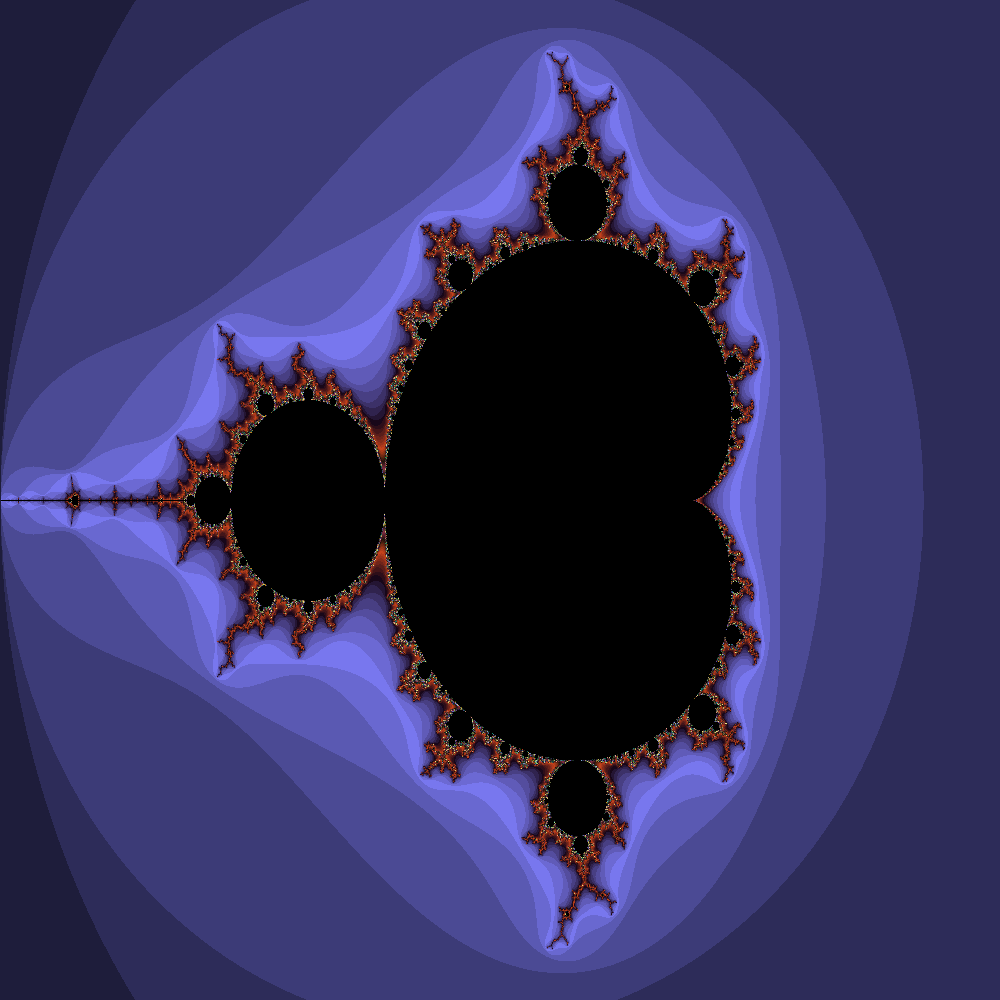
\includegraphics[scale=0.2]{Figures/mandelbrot.png}
 		\caption{An image of the Mandelbrot set generated by the code in this example.}
 		\label{fig:mandelbrotSet}
 	\end{center}
\end{figure}

Usually the image is split into ``slices'' containing a certain number of rows or columns of the image and each of these slices is assigned to a thread. Within a given slice the computation is performed pixel-by-pixel, sequentially.
The traditional way to ensure load balancing in a PThreads implementation is to split the image into small slices and to assign one of these to each thread; as soon as a thread finishes processing its slice, it gets a new one and proceeds further.
This requires additional code for managing how threads can get new work to do and it also requires synchronization, to ensure that no two threads get the same slice to process.

The implementation with HPX is much simpler: for each row of the image an \verb:async: call of the compute kernel is performed and the resulting future is stored into a vector. When all the asynchonous tasks have been created, \verb+hpx::wait_all+ is called on the vector of futures, making sure all tasks are completed before exiting.

I have tested strong scaling\footnote{How runtime improves by increasing the number of threads for a fixed problem size.} on the HPX- and PThread-based versions, with different problem sizes. I have also implemented and tested, for comparison purpose, a simple OpenMP-based version, which just parallelizes the outer loop (the row-loop). It uses dynamic scheduling for load balancing and a stride of 1 for consistency with the task grain size used with HPX.

The machine where I performed the tests has two sockets with 10 cores each, with each core exposing 2 hyperthreads. Unfortunately the machine was shared with other jobs, meaning that tests performed with a high number of threads have surely experienced preemption by the OS, artificially increasing their runtime.
However, this test is meant to roughly compare the three implementations and not to give an accurate measure on HPX's scaling capabilities. Keeping this and the aforementioned caveat in mind, we can see (Figure \ref{fig:speedupComparison}) how the performance of the HPX-based implementation is on par with the optimized PThreads-based one. On the other end we can also see how following the same approach with OpenMP does not yield the same performance: one possible explanation is that the relatively small task grain size chosen causes a relevant overhead in OpenMP.

This is clearly a toy example but it shows how HPX allows achieving good performance with simple and clean code and without any explicit optimization effort. Programmability is an important factor for making parallelism more accessible and this is surely one of the strengths of HPX.
% and neither the HPX nor the PThreads implementations have been optimized and tuned for achieving the maximum possible performance. However a certain effort was required in order to get the PThreads version right
~\\~

\subsection{Reading performance counters from the command line}
Although it is possible to access performance counter data from within the application, using the HPX API, it is also possible to make the HPX runtime print data from any performance counter to the commandline. This can be useful for debugging or for manual tuning of an HPX application.

This is achieved by passing extra flags to an HPX application and is completely handled by the runtime system, thus not requiring any change in the application code.

Available counters can be listed using the \verb/--hpx:list-counters/ flag and, if HPX was built with PAPI\footnote{Performance Application Programming Interface, which allows accessing hardware counters.} support, available PAPI events can be listed with \verb/--hpx:papi-event-info=all/.

A counter can be printed by passing the \verb/--hpx:print-counter='<counter_name>'/ argument and several counters may be specified at the same time by passing this argument multiple times.
This makes the HPX runtime system print the specified counters at the end of the execution. It is also possible to have the counters printed at regular time intervals during execution by adding the \verb/--hpx:print-counter-interval=<interval_ms>/ argument, where the interval is expressed in milliseconds.
% [\TODO Here add a couple of easy examples on how to parallelize using HPX tasks and an example on how to read a performance counter].
\begin{figure}[t]
 	\begin{center}
 		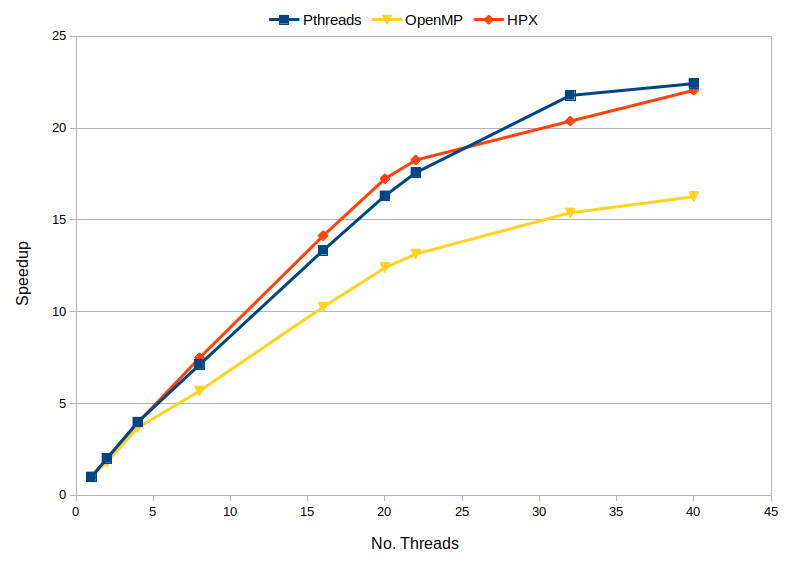
\includegraphics[scale=0.40]{Figures/mandelbrot_speedup_comparison.png}
 		\caption{Speedup comparison for PThreads, OpenMP and HPX implementations
 		% with respect to the sequential version 
 		on a $10^4$x$10^4$ image. Both the OpenMP and HPX versions use the basic features of the respective runtime system, meaning a parallelization on the row-loop (with dynamic scheduling) and an asynchronous execution for each row of the image respectively. The PThreads version instead includes a more complex logic to ensure load balancing between the threads. The results show how the HPX implementation, using basic syntax and without any specific tuning, is able to perform on par with a specifically optimized PThreads implementation. All three implementations use the same task grain size consisting of one image row.}
 		\label{fig:speedupComparison}
 	\end{center}
\end{figure}

%eof



\section{Conclusions} \label{sec:conclusions}
[\TODO Very brief recap and conclusions]


%%%%%%%%%%%%%%%%%%%%%%%%%%%%%%%%%%%%%%%%%%%%%%%%%%%%%%%%%%%%%%%%%%%%%%%%%%
% 	Acknowledgements
%%%%%%%%%%%%%%%%%%%%%%%%%%%%%%%%%%%%%%%%%%%%%%%%%%%%%%%%%%%%%%%%%%%%%%%%%%

%\section*{Acknowledgment}
%\addcontentsline{toc}{section}{Acknowledgment}

%%%%%%%%%%%%%%%%%%%%%%%%%%%%%%%%%%%%%%%%%%%%%%%%%%%%%%%%%%%%%%%%%%%%%%%%%%
% 	References
%%%%%%%%%%%%%%%%%%%%%%%%%%%%%%%%%%%%%%%%%%%%%%%%%%%%%%%%%%%%%%%%%%%%%%%%%%

% trigger a \newpage just before the given reference
% number - used to balance the columns on the last page
% adjust value as needed - may need to be readjusted if
% the document is modified later
%\IEEEtriggeratref{8}
% The "triggered" command can be changed if desired:
%\IEEEtriggercmd{\enlargethispage{-5in}}

% references section
% NOTE: BibTeX documentation can be easily obtained at:
% http://www.ctan.org/tex-archive/biblio/bibtex/contrib/doc/

% can use a bibliography generated by BibTeX as a .bbl file
% standard IEEE bibliography style from:
% http://www.ctan.org/tex-archive/macros/latex/contrib/supported/IEEEtran/bibtex
\bibliographystyle{Bib/IEEEtran}
% argument is your BibTeX string definitions and bibliography database(s)
\bibliography{Bib/IEEEabrv,Bib/references}
%
% <OR> manually copy in the resultant .bbl file
% set second argument of \begin to the number of references
% (used to reserve space for the reference number labels box)
%\begin{thebibliography}{1}
%
%\bibitem{ref:kopka}
%H.~Kopka and P.~W. Daly, \emph{A Guide to {\LaTeX}}, 3rd~ed.\hskip 1em plus
%  0.5em minus 0.4em\relax Harlow, England: Addison-Wesley, 1999.
%
%\end{thebibliography}

%%%%%%%%%%%%%%%%%%%%%%%%%%%%%%%%%%%%%%%%%%%%%%%%%%%%%%%%%%%%%%%%%%%%%%%%%%
% 	End of the document
%%%%%%%%%%%%%%%%%%%%%%%%%%%%%%%%%%%%%%%%%%%%%%%%%%%%%%%%%%%%%%%%%%%%%%%%%%

\end{document}


